% PNG export (no caption) — 2148_1.c
% Compile: pdflatex pipeline_showcase_2148_1.tex && pdftocairo -png -singlefile -r 300 ...
\documentclass[tikz,border=3pt]{standalone}
\usepackage{xcolor}
\usetikzlibrary{positioning, arrows.meta}

\definecolor{kw}{RGB}{160, 32, 160}
\definecolor{op}{RGB}{180, 60, 60}
\definecolor{num}{RGB}{20, 100, 180}
\definecolor{id}{RGB}{40, 90, 40}

\begin{document}
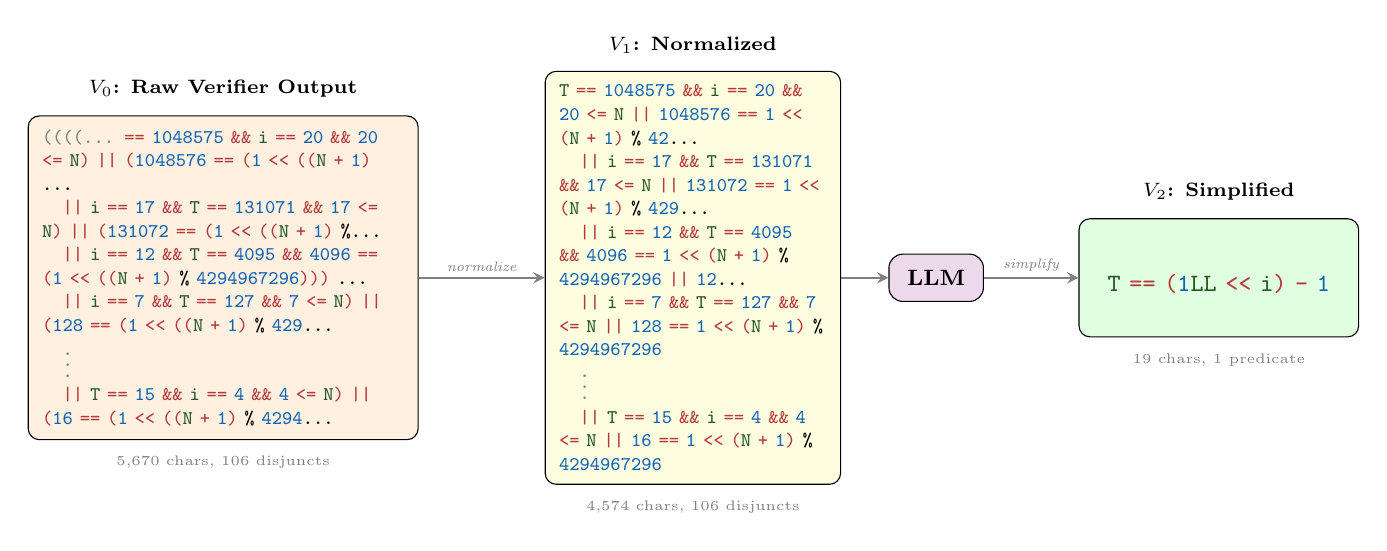
\begin{tikzpicture}[
    codebox/.style={
        draw,
        rounded corners=4pt,
        font=\ttfamily\fontsize{7}{8.5}\selectfont,
        align=left,
        fill=#1,
        inner sep=5pt
    },
    codebox/.default=white,
    llmbox/.style={
        draw,
        rounded corners=5pt,
        fill=violet!15,
        font=\footnotesize\bfseries,
        minimum height=0.6cm,
        minimum width=1.2cm
    },
    lbl/.style={font=\fontsize{7.5}{9}\selectfont\bfseries},
    sublbl/.style={font=\tiny, text=gray},
    arrowlbl/.style={font=\tiny\itshape, fill=white, inner sep=2pt}
]

% === V0: Raw Verifier Output ===
\node[codebox=orange!12, text width=4.6cm] (v0) {
\textcolor{gray}{((((...}  \textcolor{op}{==} \textcolor{num}{1048575} \textcolor{op}{\&\&} \textcolor{id}{i} \textcolor{op}{==} \textcolor{num}{20} \textcolor{op}{\&\&} \textcolor{num}{20} \textcolor{op}{<=} \textcolor{id}{N}\textcolor{op}{)} \textcolor{op}{||} \textcolor{op}{(}\textcolor{num}{1048576} \textcolor{op}{==} \textcolor{op}{(}\textcolor{num}{1} \textcolor{op}{<}\textcolor{op}{<} \textcolor{op}{(}\textcolor{op}{(}\textcolor{id}{N} \textcolor{op}{+} \textcolor{num}{1}\textcolor{op}{)} ...\\
\quad \textcolor{op}{||} \textcolor{id}{i} \textcolor{op}{==} \textcolor{num}{17} \textcolor{op}{\&\&} \textcolor{id}{T} \textcolor{op}{==} \textcolor{num}{131071} \textcolor{op}{\&\&} \textcolor{num}{17} \textcolor{op}{<=} \textcolor{id}{N}\textcolor{op}{)} \textcolor{op}{||} \textcolor{op}{(}\textcolor{num}{131072} \textcolor{op}{==} \textcolor{op}{(}\textcolor{num}{1} \textcolor{op}{<}\textcolor{op}{<} \textcolor{op}{(}\textcolor{op}{(}\textcolor{id}{N} \textcolor{op}{+} \textcolor{num}{1}\textcolor{op}{)} \%...\\
\quad \textcolor{op}{||} \textcolor{id}{i} \textcolor{op}{==} \textcolor{num}{12} \textcolor{op}{\&\&} \textcolor{id}{T} \textcolor{op}{==} \textcolor{num}{4095} \textcolor{op}{\&\&} \textcolor{num}{4096} \textcolor{op}{==} \textcolor{op}{(}\textcolor{num}{1} \textcolor{op}{<}\textcolor{op}{<} \textcolor{op}{(}\textcolor{op}{(}\textcolor{id}{N} \textcolor{op}{+} \textcolor{num}{1}\textcolor{op}{)} \% \textcolor{num}{4294967296}\textcolor{op}{)}\textcolor{op}{)}\textcolor{op}{)} ...\\
\quad \textcolor{op}{||} \textcolor{id}{i} \textcolor{op}{==} \textcolor{num}{7} \textcolor{op}{\&\&} \textcolor{id}{T} \textcolor{op}{==} \textcolor{num}{127} \textcolor{op}{\&\&} \textcolor{num}{7} \textcolor{op}{<=} \textcolor{id}{N}\textcolor{op}{)} \textcolor{op}{||} \textcolor{op}{(}\textcolor{num}{128} \textcolor{op}{==} \textcolor{op}{(}\textcolor{num}{1} \textcolor{op}{<}\textcolor{op}{<} \textcolor{op}{(}\textcolor{op}{(}\textcolor{id}{N} \textcolor{op}{+} \textcolor{num}{1}\textcolor{op}{)} \% \textcolor{num}{429}...\\
\quad \textcolor{gray}{\vdots}\\
\quad \textcolor{op}{||} \textcolor{id}{T} \textcolor{op}{==} \textcolor{num}{15} \textcolor{op}{\&\&} \textcolor{id}{i} \textcolor{op}{==} \textcolor{num}{4} \textcolor{op}{\&\&} \textcolor{num}{4} \textcolor{op}{<=} \textcolor{id}{N}\textcolor{op}{)} \textcolor{op}{||} \textcolor{op}{(}\textcolor{num}{16} \textcolor{op}{==} \textcolor{op}{(}\textcolor{num}{1} \textcolor{op}{<}\textcolor{op}{<} \textcolor{op}{(}\textcolor{op}{(}\textcolor{id}{N} \textcolor{op}{+} \textcolor{num}{1}\textcolor{op}{)} \% \textcolor{num}{4294}...\\
};
\node[lbl, above=0.1cm of v0] {$V_0$: Raw Verifier Output};
\node[sublbl, below=0.08cm of v0] {5,670 chars, 106 disjuncts};

% === V1: Normalized ===
\node[codebox=yellow!12, text width=3.4cm, right=1.6cm of v0] (v1) {
\textcolor{id}{T} \textcolor{op}{==} \textcolor{num}{1048575} \textcolor{op}{\&\&} \textcolor{id}{i} \textcolor{op}{==} \textcolor{num}{20} \textcolor{op}{\&\&} \textcolor{num}{20} \textcolor{op}{<=} \textcolor{id}{N} \textcolor{op}{||} \textcolor{num}{1048576} \textcolor{op}{==} \textcolor{num}{1} \textcolor{op}{<}\textcolor{op}{<} \textcolor{op}{(}\textcolor{id}{N} \textcolor{op}{+} \textcolor{num}{1}\textcolor{op}{)} \% \textcolor{num}{42}...\\
\quad \textcolor{op}{||} \textcolor{id}{i} \textcolor{op}{==} \textcolor{num}{17} \textcolor{op}{\&\&} \textcolor{id}{T} \textcolor{op}{==} \textcolor{num}{131071} \textcolor{op}{\&\&} \textcolor{num}{17} \textcolor{op}{<=} \textcolor{id}{N} \textcolor{op}{||} \textcolor{num}{131072} \textcolor{op}{==} \textcolor{num}{1} \textcolor{op}{<}\textcolor{op}{<} \textcolor{op}{(}\textcolor{id}{N} \textcolor{op}{+} \textcolor{num}{1}\textcolor{op}{)} \% \textcolor{num}{429}...\\
\quad \textcolor{op}{||} \textcolor{id}{i} \textcolor{op}{==} \textcolor{num}{12} \textcolor{op}{\&\&} \textcolor{id}{T} \textcolor{op}{==} \textcolor{num}{4095} \textcolor{op}{\&\&} \textcolor{num}{4096} \textcolor{op}{==} \textcolor{num}{1} \textcolor{op}{<}\textcolor{op}{<} \textcolor{op}{(}\textcolor{id}{N} \textcolor{op}{+} \textcolor{num}{1}\textcolor{op}{)} \% \textcolor{num}{4294967296} \textcolor{op}{||} \textcolor{num}{12}...\\
\quad \textcolor{op}{||} \textcolor{id}{i} \textcolor{op}{==} \textcolor{num}{7} \textcolor{op}{\&\&} \textcolor{id}{T} \textcolor{op}{==} \textcolor{num}{127} \textcolor{op}{\&\&} \textcolor{num}{7} \textcolor{op}{<=} \textcolor{id}{N} \textcolor{op}{||} \textcolor{num}{128} \textcolor{op}{==} \textcolor{num}{1} \textcolor{op}{<}\textcolor{op}{<} \textcolor{op}{(}\textcolor{id}{N} \textcolor{op}{+} \textcolor{num}{1}\textcolor{op}{)} \% \textcolor{num}{4294967296}\\
\quad \textcolor{gray}{\vdots}\\
\quad \textcolor{op}{||} \textcolor{id}{T} \textcolor{op}{==} \textcolor{num}{15} \textcolor{op}{\&\&} \textcolor{id}{i} \textcolor{op}{==} \textcolor{num}{4} \textcolor{op}{\&\&} \textcolor{num}{4} \textcolor{op}{<=} \textcolor{id}{N} \textcolor{op}{||} \textcolor{num}{16} \textcolor{op}{==} \textcolor{num}{1} \textcolor{op}{<}\textcolor{op}{<} \textcolor{op}{(}\textcolor{id}{N} \textcolor{op}{+} \textcolor{num}{1}\textcolor{op}{)} \% \textcolor{num}{4294967296}\\
};
\node[lbl, above=0.1cm of v1] {$V_1$: Normalized};
\node[sublbl, below=0.08cm of v1] {4,574 chars, 106 disjuncts};

% === LLM ===
\node[llmbox, right=0.6cm of v1] (llm) {LLM};

% === V2: Simplified ===
\node[codebox=green!12, right=1.2cm of llm, minimum height=1.5cm, text width=3.2cm, align=center, font=\ttfamily\small] (v2) {
\vfill
\textcolor{id}{T} \textcolor{op}{==} \textcolor{op}{(}\textcolor{num}{1}\textcolor{id}{LL} \textcolor{op}{<}\textcolor{op}{<} \textcolor{id}{i}\textcolor{op}{)} \textcolor{op}{-} \textcolor{num}{1}
\vfill
};
\node[lbl, above=0.1cm of v2] {$V_2$: Simplified};
\node[sublbl, below=0.08cm of v2] {19 chars, 1 predicate};

% === Arrows ===
\draw[->, >=stealth, thick, gray] (v0.east) -- (v1.west) node[arrowlbl, midway, above] {normalize};
\draw[->, >=stealth, thick, gray] (v1.east) -- (llm.west);
\draw[->, >=stealth, thick, gray] (llm.east) -- (v2.west) node[arrowlbl, midway, above] {simplify};

\end{tikzpicture}
\end{document}
